\chapter{Dynamic Causal Modeling for fMRI \label{Chap:DCM_fmri}}


\section{Theoretical background}
Dynamic Causal Modelling (DCM) is a method for making inferences about neural processes that underlie measured time series, e.g. fMRI data.  The general idea is to estimate the parameters of a reasonably realistic neuronal system model such that the predicted blood oxygen level dependent (BOLD) signal, which results from converting the modeled neural dynamics into hemodynamic responses, corresponds as closely as possible to the observed BOLD time series.  This section gives a short introduction to the theoretical background of DCM for fMRI; details can be found in \cite{dcm}.  Note that DCMs can be formulated, in principle, for any measurement technique.  Depending on the spatio-temporal properties of a given measurement technique, one needs to define an adequate state equation and an observation model. See Fig~\ref{fig1} for a summary of the differences between DCM implementations for fMRI and Event-Related Potentials (ERPs).

\begin{figure}[ht]
\begin{center}
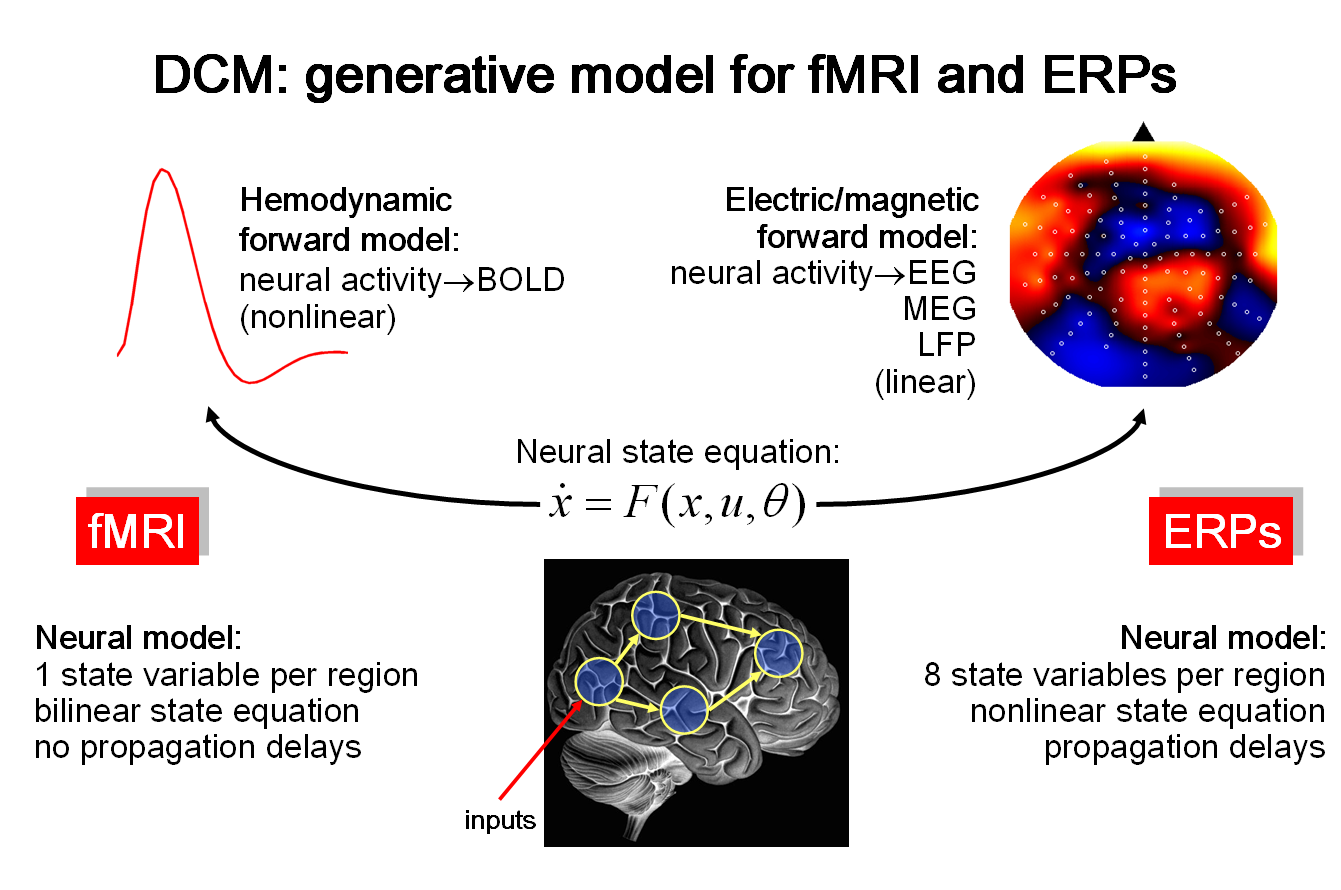
\includegraphics[width=100mm]{dcm/Fig1}
\caption{\em A schematic overview of the differences between between the DCM implementations for fMRI and ERPs (as measured by EEG or MEG).  Whereas the state equation of DCM for fMRI is bilinear and uses only a single state variable per region, that for ERPs is more complex and requires 8 state variables per region.  Moreover, DCM for ERPs models the delays of activity propagation between areas.  At the level of the observation model, DCM for fMRI is more complex than DCM for ERPs.  While the former uses a non-linear model of the hemodynamic response that contains a cascade of differential equations with five state variables per region, the latter uses a simple linear model for predicting observed scalp data.\label{fig1}}
\end{center}
\end{figure}

As in state-space models, two distinct levels constitute a DCM (see Figure~\ref{fig2}).  The hidden level, which cannot be directly observed using fMRI, represents a simple model of neural dynamics in a system of $k$ coupled brain regions.  Each system element $i$ is represented by a single state variable $z_i$, and the dynamics of the system is described by the change of the neural state vector  over time.

The neural state variables do not correspond directly to any common neurophysiological measurement (such as spiking rates or local field potentials) but represent a summary index of neural population dynamics in the respective regions.  Importantly, DCM models how the neural dynamics are driven by external perturbations that result from experimentally controlled manipulations.  These perturbations are described by means of external inputs $u$ that enter the model in two different ways:  they can elicit responses through direct influences on specific regions (``driving'' inputs, e.g. evoked responses in early sensory areas) or they can change the strength of coupling among regions (``modulatory'' inputs, e.g. during learning or attention).

Overall, DCM models the temporal evolution of the neural state vector, i.e. , as a function of the current state, the inputs $u$ and some parameters  that define the functional architecture and interactions among brain regions at a neuronal level ($n$  denotes ``neural''):
\begin{equation}
\left[ \begin{array}{l}
  \dot{z}_1 \\
  \dot{z}_2 \\
  .. \\
  \dot{z}_k \\  \end{array} \right] = \dot{z}= \frac{dz}{dt} = F(z,u,\theta^n)
\end{equation}
In this neural state equation, the state $z$ and the inputs $u$ are time-dependent whereas the parameters are time-invariant.  In DCM, $F$ has the bilinear form
 \begin{equation}
\dot{z}=Az+\sum_{j=1}^m u_j B_j z + Cu
\end{equation}
The parameters of this bilinear neural state equation, $\theta^n=\{A,B_1,...,B_m,C\}$, can be expressed as partial derivatives of $F$:
\begin{eqnarray}
A & = & \frac{\partial F}{\partial z} = \frac{\partial \dot{z}}{\partial z} \\ \nonumber
B_j & = & \frac{\partial^2 F}{\partial z \partial u_j} = \frac{\partial}{\partial u_j}\frac{\partial \dot{z}}{\partial z}  \\ \nonumber
C & = & \frac{\partial F}{\partial u}
\end{eqnarray}
These parameter matrices describe the nature of the three causal components which underlie the modeled neural dynamics:  (i) context-independent effective connectivity among brain regions, mediated by anatomical connections ($k \times k$ matrix $A$), (ii) context-dependent changes in effective connectivity induced by the $j$th input $u_j$ ($k \times k$ matrices $B_1$, ..., $B_m$), and (iii) direct inputs into the system that drive regional activity ($k \times m$ matrix $C$).  As will be demonstrated below, the posterior distributions of these parameters can inform us about the impact that different mechanisms have on determining the dynamics of the model.  Notably, the distinction between ``driving'' and ``modulatory'' is neurobiologically relevant: driving inputs exert their effects through direct synaptic responses in the target area, whereas modulatory inputs change synaptic responses in the target area in response to inputs from another area.  This distinction represents an analogy, at the level of large neural populations, to the concept of driving and modulatory afferents in studies of single neurons.

\begin{figure}[ht]
\begin{center}
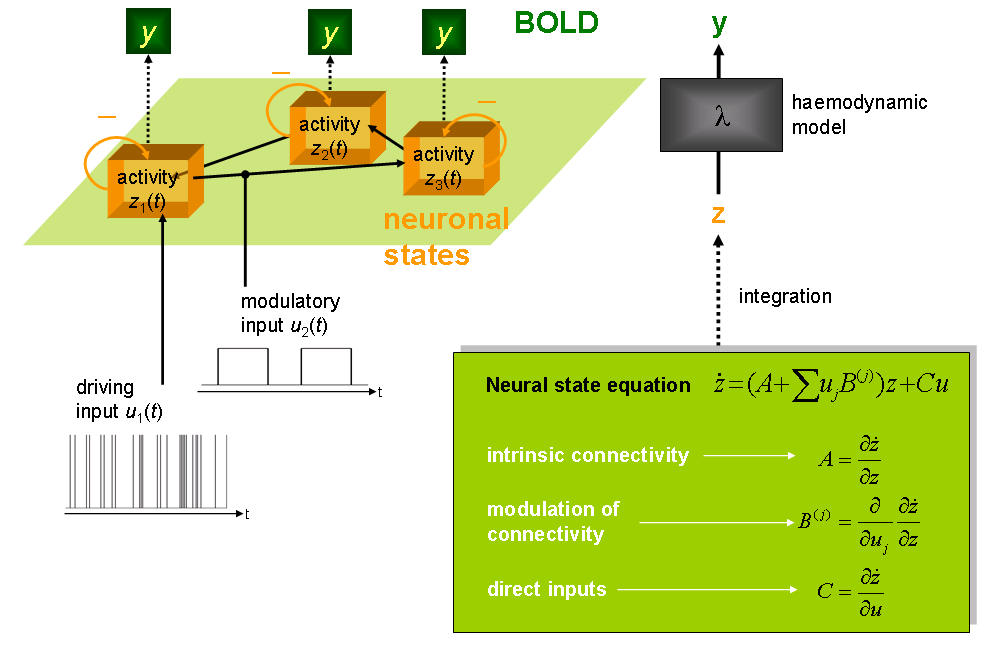
\includegraphics[width=130mm]{dcm/Fig2}
\caption{\em Schematic summary of the conceptual basis of DCM.  The dynamics in a system of interacting neuronal populations (orange boxes), which are not directly observable by fMRI, is modeled using a bilinear state equation (grey box).  Integrating the state equation gives predicted neural dynamics ($z$) that enter a model of the hemodynamic response ($\lambda$) to give predicted BOLD responses ($y$) (green boxes).  The parameters at both neural and hemodynamic levels are adjusted such that the differences between predicted and measured BOLD series are minimized.  Critically, the neural dynamics are determined by experimental manipulations.  These enter the model in the form of ``external'' or ``driving'' inputs.  Driving inputs ($u_1$; e.g. sensory stimuli) elicit local responses directly that are propagated through the system according to the intrinsic connections.  The strengths of these connections can be changed by modulatory inputs ($u_2$; e.g. changes in cognitive set, attention, or learning).\label{fig2}}
\end{center}
\end{figure}

DCM combines this model of neural dynamics with a biophysically plausible and experimentally validated hemodynamic model that describes the transformation of neuronal activity into a BOLD response.  This so-called ``Balloon model'' was initially formulated by Buxton and colleagues and later extended by \cite{balloon}.  Briefly summarized, it consists of a set of differential equations that describe the relations between four hemodynamic state variables, using five parameters ($\theta^h$).  More specifically, changes in neural activity elicit a vasodilatory signal that leads to increases in blood flow and subsequently to changes in blood volume $v$ and deoxyhemoglobin content $q$.  The predicted BOLD signal $y$ is a non-linear function of blood volume and deoxyhemoglobine content. Details of the hemodynamic model can be found in other publications \cite{balloon}.
By combining the neural and hemodynamic states into a joint state vector x and the neural and hemodynamic parameters into a joint parameter vector $\theta=[\theta^n, \theta^h]^T$, we obtain the full forward model that is defined by the neural and hemodynamic state equations
\begin{eqnarray}
\dot{x} & = & F(x,u,\theta) \\ \nonumber
y & = & \lambda(x)
\end{eqnarray}
For any given set of parameters $\theta$ and inputs $u$, the joint state equation can be integrated and passed through the output nonlinearity $\lambda$ to give a predicted BOLD response $h(u,\theta)$.  This can be extended to an observation model that includes observation error $e$ and confounding effects $X$ (e.g. scanner-related low-frequency drifts):
\begin{equation}
y = h(u,\theta) + X \beta + e
\end{equation}
This formulation is the basis for estimating the neural and hemodynamic parameters from the measured BOLD data, using a fully Bayesian approach with empirical priors for the hemodynamic parameters and conservative shrinkage priors for the neural coupling parameters.

Details of the parameter estimation scheme, which rests on a Fisher scoring gradient ascent scheme with Levenburg-Marquardt regularisation, embedded in an expectation maximization (EM) algorithm, can be found in the original DCM publication (Friston et al. 2003).  In brief, under Gaussian assumptions about the posterior distributions, this scheme returns the posterior expectations $\eta_{\theta | y}$ and posterior covariance  $C_{\theta | y}$ for the parameters as well as hyperparameters for the covariance of the observation noise, $C_e$.

After fitting the model to measured BOLD data, the posterior distributions of the parameters can be used to test hypotheses about the size and nature of effects at the neural level.  Although inferences could be made about any of the parameters in the model, hypothesis testing usually concerns context-dependent changes in coupling (i.e. specific parameters from the $B$ matrices; see Fig.~\ref{fig6}).  As will be demonstrated below, at the single-subject level, these inferences concern the question of how certain one can be that a particular parameter or, more generally, a contrast of parameters, $c^T \eta_{\theta | y}$, exceeds a particular threshold  $\gamma$ (e.g. zero).

Under the assumptions of the Laplace approximation, this is easy to test ($\Phi_N$ denotes the cumulative normal distribution):
\begin{equation}
p(c^T \eta_{\theta | y} > \gamma) = \Phi_N \left(\frac{c^T \eta_{\theta | y} - \gamma}{c^T C_{\theta | y} c} \right)
\end{equation}
For example, for the special case $c^T \eta_{\theta | y} = \gamma$ the probability is $p(c^T \eta_{\theta | y} > \gamma)=0.5$, i.e. it is equally likely that the parameter is smaller or larger than the chosen threshold $\gamma$.
We conclude this section on the theoretical foundations of DCM by noting that the parameters can be understood as rate constants (units: $1/s = Hz$) of neural population responses that have an exponential nature.  This is easily understood if one considers that the solution to a linear ordinary differential equation of the form $\dot{z}=Az$ is an exponential function (see Fig. ~\ref{fig3}).
\begin{figure}[ht]
\begin{center}
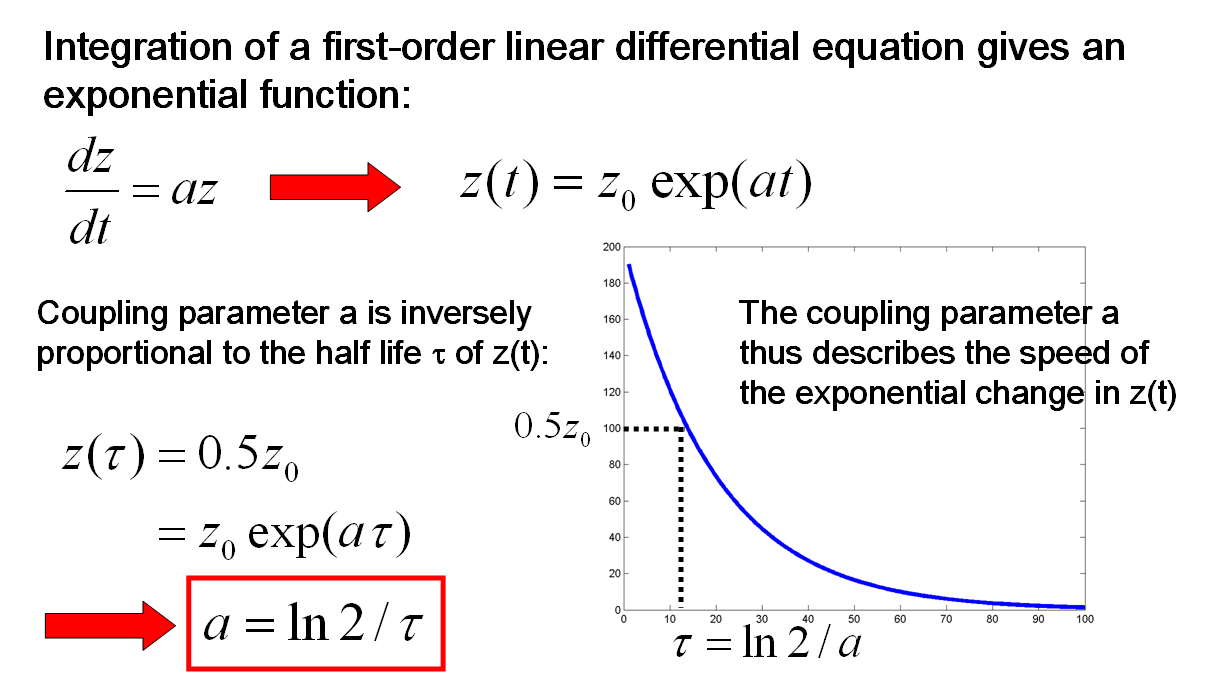
\includegraphics[width=120mm]{dcm/Fig3}
\caption{\em A short mathematical demonstration, using a simple linear first-order differential equation as an example, explaining why the coupling parameters in a DCM are inversely proportional to the half-life of the modelled neural responses and are therefore in units of 1/s = Hertz.\label{fig3}}
\end{center}
\end{figure}

\section{Bayesian model selection \label{mc}}

A generic problem encountered by any kind of modeling approach is the question of model selection:  given some observed data, which of several alternative models is the optimal one?  This problem is not trivial because the decision cannot be made solely by comparing the relative fit of the competing models.  One also needs to take into account the relative complexity of the models as expressed, for example, by the number of free parameters in each model.

Model complexity is important to consider because there is a trade-off between model fit and generalizability (i.e. how well the model explains different data sets that were all generated from the same underlying process).  As the number of free parameters is increased, model fit increases monotonically whereas beyond a certain point model generalizability decreases.  The reason for this is ``overfitting'':  an increasingly complex model will, at some point, start to fit noise that is specific to one data set and thus become less generalizable across multiple realizations of the same underlying generative process.

    Therefore, the question ``What is the optimal model?'' can be reformulated more precisely as ``What is the model that represents the best balance between fit and complexity?''. In a Bayesian context, the latter question can be addressed by comparing the evidence, $p(y|m)$, of different models. According to Bayes theorem
\begin{equation}
p(\theta|y,m) = \frac{p(y|\theta,m)p(\theta|m)}{p(y|m)}
\end{equation}
the model evidence can be considered as a normalization constant for the product of the likelihood of the data and the prior probability of the parameters, therefore
\begin{equation}
p(y|m) = \int p(\theta|y,m) p(\theta|m) d\theta
\end{equation}
Here, the number of free parameters (as well as the functional form) are considered by the integration.  Unfortunately, this integral cannot usually be solved analytically, therefore an approximation to the model evidence is needed. One such approximation used by DCM, and many other models in SPM, is to make use of the Laplace approximation~\footnote{This should perhaps more correctly be referred to as a fixed-form variational approximation, where the fixed form is chosen to be a Gaussian. The model evidence is approximated by the negative free energy, $F$.}.

As shown in \cite{cdcm}, this yields the following expression for the natural logarithm ($ln$) of the model evidence ( $\eta_{\theta | y}$ denotes the posterior mean, $C_{\theta | y}$ is the posterior covariance of the parameters, $C_e$  is the error covariance, $\theta_p$ is the prior mean of the parameters, and $C_p$ is the prior covariance):
\begin{eqnarray}
ln p(y|m) & = & accuracy(m) - complexity (m) \\ \nonumber
& = & \left[ -\frac{1}{2} ln |C_e| - \frac{1}{2} (y-h(u,\eta_{\theta | y}))^T C_e^{-1} (y-h(u,\eta_{\theta | y}))\right] \\ \nonumber
& - & \left[ \frac{1}{2} ln |C_p| -\frac{1}{2}ln |C_{\theta | y}| + \frac{1}{2} (\eta_{\theta | y}-\theta_p)^T C_p^{-1} (\eta_{\theta | y}-\theta_p) \right]
\end{eqnarray}

This expression properly reflects the requirement, as discussed above, that the optimal model should represent the best compromise between model fit (accuracy) and model complexity.  The complexity term depends on the prior density, for example, the prior covariance of the intrinsic connections.  

Two models can then be compared using the Bayes factor:
\begin{equation}
BF_{ij} = \frac{p(y|m_i)}{p(y|m_j)}
\end{equation}
Given uniform priors over models, the posterior probability for model $i$ is greater 0.95 if $BF_{ij}$ is greater than twenty.

This results in a robust procedure for deciding between competing hypotheses represented by different DCMs. These hypotheses can concern any part of the structure of the modeled system, e.g. the pattern of intrinsic connections or which inputs affect the system and where they enter. Note, however, that this comparison is only valid if the data $y$ are identical in all models.  This means that in DCM for fMRI, where the data vector results from a concatenation of the time series of all areas in the model, only models can be compared that contain the same areas. Therefore, model selection cannot be used to address whether or not to include a particular area in the model.  In contrast, in DCM for ERPs, the data measured at the sensor level are independent of how many neuronal sources are assumed in a given model.  Here, model selection could also be used to decide which sources should be included.

\section{Practical example}

The following example refers to the ``attention to visual motion'' data set available from the SPM web site\footnote{Attention to visual motion dataset: \url{http://www.fil.ion.ucl.ac.uk/spm/data/attention/}}. This data set was obtained by Christian Buchel and is described in \cite{buchel97}.  Note that the data available from the web have been pre-processed using SPM99, therefore ensure \texttt{flip} is set to \texttt{1} in the \texttt{spm\_flip\_analyze\_images.m} file before proceeding further.

Making a DCM requires two ingredients: (i) a design matrix and (ii) the time series, stored in VOI files.  The regressors of the design matrix define the inputs for the DCM.  Note that this means that the design matrix that is optimal for a given DCM is often somewhat different than the one for the corresponding GLM. DCM does not require the design matrix to be part of an estimated model, however. It just needs to be defined.

\subsection{Defining the GLM}
The present experiment consisted of 4 conditions: (i) fixation (F), (ii) static (S, non-moving dots), (iii) no attention (N, moving dots but no attention required), (iv) attention (A). The GLM analyses by Christian showed that activity in area V5 was not only enhanced by moving stimuli, but also by attention to motion.  In the following, we will try to model this effect in V5, and explain it as a context-dependent modulation or ``enabling'' of V5 afferents, using a DCM. First, we need to set up the GLM analysis and extract our time series from the results. In this example, we want to use the same design matrix for GLM and DCM, therefore we recombine the above regressors to get the following three conditions:
\begin{enumerate}
\item{{\bf photic}: this comprises all conditions with visual input, i.e. S, N, and A.}
\item{{\bf motion}: this includes all conditions with moving dots, i.e. N and A.}
\item{{\bf attention}: this includes the attention-to-motion (A) condition only.}
\end{enumerate}
Now we need to define and estimate the GLM. See chapters \ref{Chap:fmri_spec} and \ref{Chap:fmri_est} on how to do this. Here are the relevant details for this data set that you need to set up the GLM (this information can also be found online\footnote{\url{ftp://ftp.fil.ion.ucl.ac.uk/spm/data/attention/README_GLM_DCM.txt}}
note this web site describes the analysis for SPM2).
\begin{itemize}
\item{The onsets for the conditions can be found in the file factors.mat.  They are named phot (photic), mot (motion) and att (attention) and are defined in scans (not seconds!).  They are blocks of 10 TRs each.}
\item{The TR is 3.22 seconds.}
\item{There are 360 scans.}
\end{itemize}

\subsection{Extracting time series}

Once you have specified and estimated the GLM, you should define t-contrasts that test for photic, motion, and attention, respectively. These serve to locate areas that show effects due to visual stimulation (e.g. in V1), motion (e.g. V5) and attention (e.g. V5 and superior parietal cortex, SPC). Because V5 shows both motion and attention effects, it is useful to mask the motion-contrast inclusively with the attention-contrast when extracting time series for V5. You should also compute the usual ``effects of interest'' F-contrast, this is needed for mean-correcting the extracted time series (see below). Here is a step-by-step example for extracting the V5 time series:
\begin{enumerate}
\item{Press ``Results''.}
\item{Select the \texttt{SPM.mat} file.}
\item{Choose the t-contrast for the motion condition.}
\item{Mask with other contrasts: Yes}
\item{Choose the t-contrast for the attention condition.}
\item{Mask inclusively and choose a threshold of $p \leq 0.05$ uncorrected.}
\item{Select the local maximum of a blob that looks V5-ish, e.g. -45/-81/-9 (by overlaying the activations onto the normalised structural image you should be able to identify V5 more easily).}
\item{Press the ``VOI'' button.}
\item{Name of region: V5}
\item{Adjust data for: effects of interest (this mean-corrects the time series)}
\item{VOI definition: sphere}
\item{VOI radius(mm): e.g. 8 mm}
\end{enumerate}
SPM now computes the first principal component of the time series from all voxels included in the sphere.  The result is stored (together with the original time series) in a file named \verb!VOI_V5_1.mat! in the working directory.  You can now proceed to select time series for V1 (using the ``photic'' contrast) and SPC (using the ``attention'' contrast).  For this example, we selected -6/-84/-6 for V1 and -18/-57/66 for SPC.

\subsection{Specifying and estimating the DCM}

Now we have defined the inputs (via the design matrix) and the time series, we are ready to build the DCM. We will look at a simplified version of the model described in \cite{dcm}.  In our example here, we will model a hierarchically connected system comprising V1, V5 and SPC, i.e. reciprocal connections between V1-V5 and V5-SPC, but not between V1-SPC. We will assume that (i) V1 is driven by any kind of visual stimulation (direct input ``photic''), (ii) motion-related responses in V5 can be explained through an increase in the influence of V1 onto V5 whenever the stimuli are moving (i.e. ``motion'' acts as modulatory input onto the $V1 \rightarrow V5$ connection) and (iii) attention enhances the influence of SPC onto V5 (i.e. ``attention'' acts as modulatory input onto the $SPC \rightarrow V5$ connection). This DCM is shown schematically in Figure~\ref{bwd}, and can be made
\begin{figure}[ht]
\begin{center}
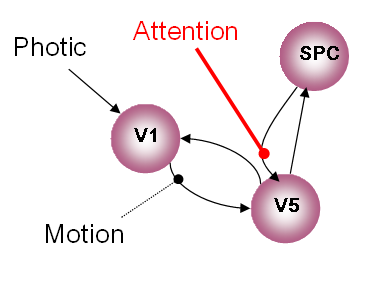
\includegraphics[width=100mm]{dcm/dcm_mod_bwd}
\caption{\em DCM with attentional modulation of backwards connection. Dotted lines denote modulatory connections.\label{bwd}}
\end{center}
\end{figure}
as follows:
\begin{enumerate}
\item{Press the \texttt{DCM} button.}
\item{Choose ``specify''.}
\item{Select the \texttt{SPM.mat} file you just created when specifying the GLM.}
\item{Name for \verb!DCM_???.mat!:  e.g. \verb!mod_bwd! (for ``attentional modulation of backward connection'')}
\item{Select all VOIs in order \verb!VOI_V1_1, VOI_V5_1, VOI_SPC_1!}
\item{Include Photic: Yes}
\item{Include Motion: Yes}
\item{Include Attention: Yes}
\item{Define the following intrinsic connections: V1 to V5, V5 to V1, V5 to SPC, SPC to V5, i.e. a hierarchy with reciprocal connections between neighbouring areas. Note that the columns specify the source of the connection and the rows specify its target. Your connectivity matrix should look like the one in Fig.~\ref{fig4}.}
\item{Specify Photic as a driving input into V1.  See Fig.~\ref{fig5}}
\item{Specify Motion to modulate the connection from V1 to V5.  See Fig.~\ref{fig6}}
\item{Specify Attention to modulate the connection from SPC to V5.  See Fig.~\ref{fig7}}
\item{Say No for ``Nonlinear DCM?''}
\item{Specify slice timings for each area. This is a new option described in \cite{sjk_dcm_slicetiming}. The default values are set to the last slice of the data, which was the default in the original DCM version. For sequential (as opposed to interleaved) data, this modelling option allows to use DCM in combination with any TR (slice timing differences). Here, we proceed with the default values.}
\item{Enter \texttt{0.04} for ``Echo Time, TE[s]''.}
\end{enumerate}
A polite ``Thank you'' completes the model specification process.

\begin{figure}[ht]
\begin{center}
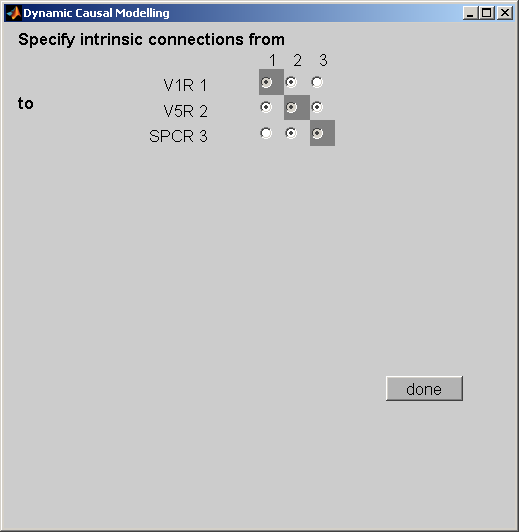
\includegraphics[width=70mm]{dcm/Fig4}
\caption{\em Filled circles define the structure of the intrinsic connections $C$ such that eg. there are no connections from V1R to SPCR or from SPCR to V1R. See also Fig~\ref{bwd}.\label{fig4}}
\end{center}
\end{figure}
\begin{figure}[ht]
\begin{center}
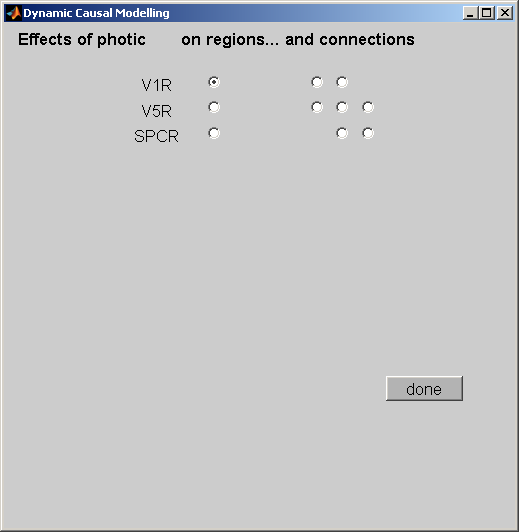
\includegraphics[width=70mm]{dcm/Fig5}
\caption{\em The filled circle specifies that the input `phot' connects to region V1R. See also Fig~\ref{bwd}.\label{fig5}}
\end{center}
\end{figure}
\begin{figure}[ht]
\begin{center}
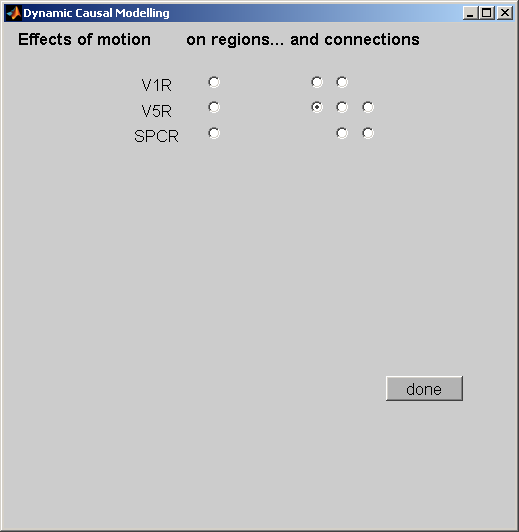
\includegraphics[width=70mm]{dcm/Fig6}
\caption{\em The filled circle indicates that the input variable `mot' can modulate the connection from V1R to V5R. This specifies a `modulatory' connection. See also Fig~\ref{bwd}.\label{fig6}}
\end{center}
\end{figure}
\begin{figure}[ht]
\begin{center}
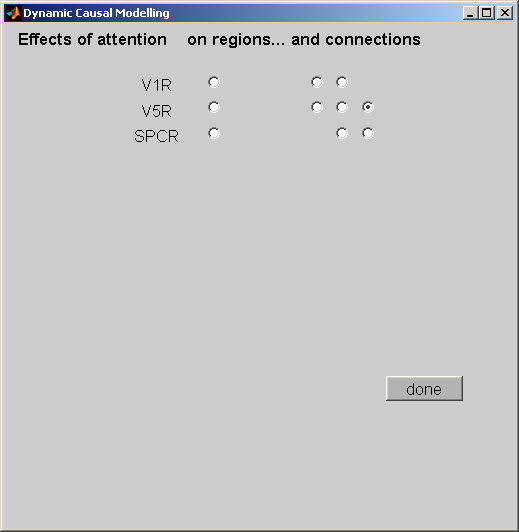
\includegraphics[width=70mm]{dcm/Fig7}
\caption{\em The filled circle indicates that attention can modulate the connection from SPCR to V5R. See also Fig~\ref{bwd}.\label{fig7}}
\end{center}
\end{figure}

You can now estimate the model parameters, either by pressing the DCM button again and choosing ``estimate'', or by typing \verb!spm_dcm_estimate('DCM_mod_bwd')! from the \matlab\ command line.  Once this is completed, you can review the results as follows:
\begin{enumerate}
\item{Press the DCM button.}
\item{Choose ``review''.}
\item{Select \verb!DCM_mod_bwd!}
\item{Threshold: 0}
\end{enumerate}
Now you have multiple options, e.g. you can revisit the fit of the model (``Outputs'') or look at the parameter estimates for the intrinsic connections (``Intrinsic connections'') or for the parameters associated with the driving or modulatory inputs (``Effects of Photic'', ``Effects of Motion'', ``Effects of Attention'').

Also, you can use the ``Contrasts'' option to determine how confident you can be that a contrast of certain parameter estimates exceeds the threshold you chose in step 4.
Of course, you can also explore the model results at the level of the \matlab\ command line by loading the model and inspecting the parameter estimates directly.  These can be found in \texttt{DCM.A} (intrinsic connections), \texttt{DCM.B} (modulatory inputs) and \texttt{DCM.C} (driving inputs).

\subsection{Comparing models}

Let us now specify an alternative model and compare it against the one that we defined and estimated above. The change that we are going to make is to assume that attention modulates the $V1 \rightarrow V5$ connection (as opposed to the $SPC \rightarrow V5$ connection in the previous model). For defining this model, you repeat all the steps from the above example, the only differences being that the model gets a new name (e.g. \verb!mod_fwd!) and that attention now acts on the forward connection. This DCM is shown schematically in Figure~\ref{fwd}.
\begin{figure}[ht]
\begin{center}
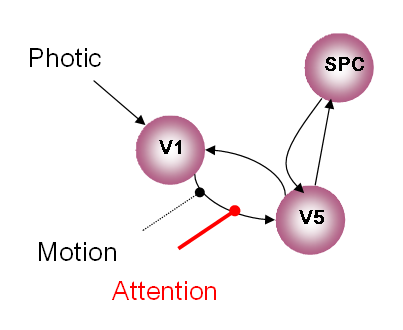
\includegraphics[width=100mm]{dcm/dcm_mod_fwd}
\caption{\em DCM with attentional modulation of forwards connection. Dotted lines denote modulatory connections.\label{fwd}}
\end{center}
\end{figure}
Once you have estimated this new model, you can perform a Bayesian model comparison as follows:
\begin{enumerate}
\item{Press the ``DCM'' button.}
\item{Choose ``compare''.}
\item{Number of models to compare: 2}
\item{Select the two models, e.g. in the order \verb!DCM_mod_bwd! and \verb!DCM_mod_fwd!.}
\end{enumerate}

The Graphics window, Fig.~\ref{fig8}, now shows a bar plot of the model evidence. You can see that our second model is better than the first one. 

\begin{figure}[ht]
\begin{center}
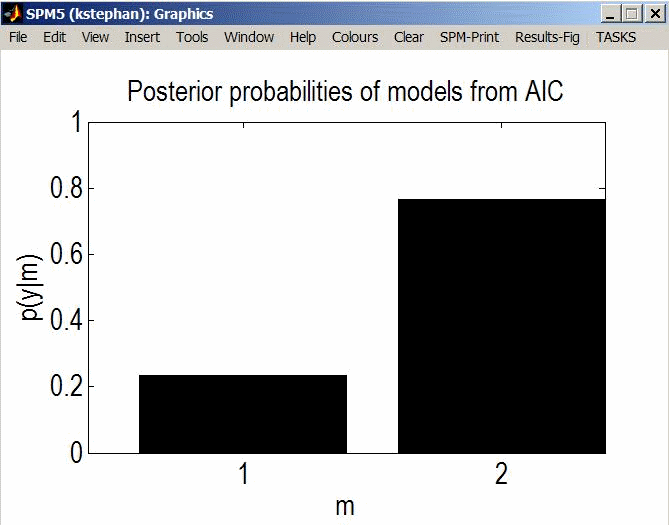
\includegraphics[width=100mm]{dcm/Fig8}
\caption{\em Model 2 (shown in Fig~\ref{fwd}) is preferred to model 1 (shown in Fig~\ref{bwd}).\label{fig8}}
\end{center}
\end{figure}
